\documentclass[a4paper,twoside,10pt]{article}

\usepackage[left=2.5cm,right=2.5cm,top=0.5cm,bottom=2.5cm]{geometry}
\usepackage{graphicx,type1cm,eso-pic,color}
\usepackage{url}
\usepackage[latin1]{inputenc}
\usepackage[T1]{fontenc}
% Extension postscript
\usepackage{graphicx}
\usepackage{color}
\usepackage{amsmath}
\usepackage{amsfonts}
\usepackage[english,french]{babel}
\usepackage[toc,page]{appendix} 
\usepackage{palatino}
\usepackage{color}
\usepackage{listings}
\usepackage{ifthen}
\usepackage{tabularx}
\usepackage{array}
\usepackage{subfigure}
\usepackage{rotating}
\bibliographystyle{unsrt}
\usepackage{lastpage} 
\usepackage{multirow}
\usepackage{fancyhdr}
\newcommand{\topfigrule}{%
  \vspace*{5pt}\hrule\vspace{-5pt}}

\newcommand\musec{\mu\text{s}}

\title{Documentation maquette IJK + Front-tracking}

\author{Benoit Mathieu et Guillaume Bois}
\begin{document}
\selectlanguage{french}
\maketitle
\section{Conventions}
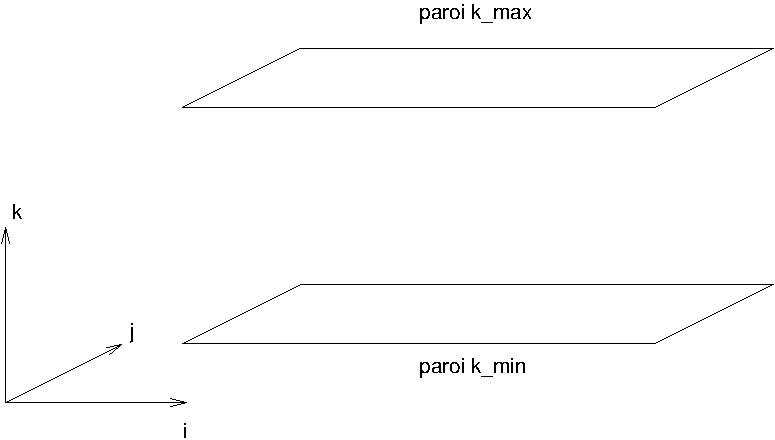
\includegraphics{conventions}
\section{ A propos du solveur multigrille}
\begin{itemize}
 \item Le seuil du solveur grossier doit �tre inf�rieur au seuil du solveur global
(par exemple seuil gcp � $10^{-10}$ pour un seuil global � $10^{-9}$)
\end{itemize}
\begin{verbatim}
multigrid_solver {
    solver_precision mixed
    # Liste des operateurs de deraffinement, le nombre d'operateurs
      donne le nombre de niveaux.
      4 operateurs => niveaux 0 (origine), 1, 2, 3, 4 (niveau grossier) 
      Ici, niveau grossier aura 2^4 fois moins de mailles par direction que
      le niveau 0 (16 fois) #
    coarsen_operators 4
      Coarsen_Operator_Uniform {  }
      Coarsen_Operator_Uniform {  }
      Coarsen_Operator_Uniform {  } 	
      Coarsen_Operator_Uniform {  } 	
    # parametre d'optimisation "temporal blocking" #
    ghost_size 1
    pre_smooth_steps 1 7
    smooth_steps 1 7
    relax_jacobi 1 0.7
    # solveur utilise pour le maillage le plus grossier (niveau 4) avec seuil #
    solveur_grossier GCP { impr seuil 1e-10  precond ssor { omega 1.5 } }
    # seuil du solveur multigrille global: #
    seuil 1e-8
    nb_full_mg_steps 2 20 1
    impr
  }
\end{verbatim}
\subsection{temporal blocking}
Le temporal blocking est une optimisation de l'algorithme Jacobi qui fait plusieurs it�rations
de lissage de Jacobi en parcourant une seule fois les champs d'entree et de sortie.
Pour cela on a besoin de plusieurs couches de mailles fantomes (ghost\_size), autant que
de passe simultan�es. Sur les processeurs r�cents, l'optimum est ghost\_size=4 � 6 pour des
maillages de taille 32 � 64 de c�t� en i et j, par processeur.
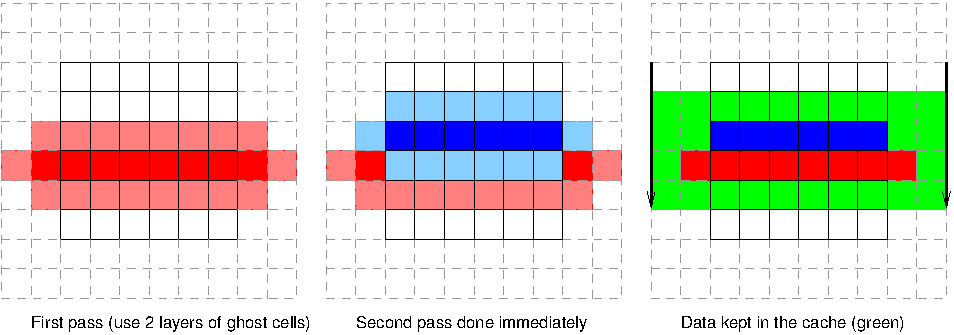
\includegraphics{expose_pici2_25_03_2011/jacobi_sweep}
Voir pr�sentation pici2 du 25/03/2011.

Attention: le parametre ghost\_size ne peut pas etre plus grand que la taille du maillage le plus grossier sur un processeur.
\section{Quelques infos sur le Front-tracking}

Il y a un objet maillage par proc. 
La m�thode \verb maillage.cree_sommets_virtuels() est appel�e en m�me temps sur tous les processeurs;

La suppression des facettes inutiles se fait lors de la r��valuation de l'indicatrice. 

\subsection{Classe Descripteur\_FT}
Classe envoyant la liste des sommets/facettes aux autres processeurs.

Il y a 2 \verb Desc_Structure_FT : un pour les sommets et un pour les facettes : 
\verb desc_sommets_ et \verb#desc_facettes_#

Chacun poss�de un espace virtuel et un espace distant (les espaces sont de type Descripteur\_FT). Le virtuel est celui qu'il re�oit d'autres processeurs; le distant est celui qu'il envoie aux autres. 

\begin{verbatim}
PROC1:                                   
 doit envoyer le sommet 0 au processeur 2
 doit envoyer le sommet 4 au processeur 2


PROC2:
 doit recevoir, dans l'ordre, du processeur 1:
    le premier sommet recu dans le sommet 3,  
    le deuxieme sommet recu dans le sommet 4  

PROC1:
maillage.desc_sommets_.espace_distant_.elements_[2] =
   { 0, 4 }                                          

PROC2:
maillage.desc_sommets_.espace_virtuel_.elements_[1] =
   { 3, 4 }


sur le processeur 1:
appeler maillage.creer_sommets_virtuels(
   liste_sommets = { 0, 4 }
   liste_pe = { 2, 2 }
)
c'est une methode parallele, le proc 1 va envoyer des donnees
et le proc 2 va en attendre en reception,
il faut donc appeler la methode sur le proc2  aussi, en meme temps:

PROC2:
maillage.creer_sommets_virtuels(
   liste_sommets= {}
   liste_pe = {}
)
\end{verbatim}


\subsection{Liste des classes Front-tracking utilis�es et/ou modifi�es}
\begin{itemize}
 \item Intersections\_Elem\_Facettes et Intersections\_Elem\_Facettes\_Data: base de donn�es contenant pour chaque
  maille volumique la liste des facettes qui la traverse, et pour chaque facette
  la liste des mailles volumiques travers�es. Pour chaque couple, on conna�t le
  barycentre de la surface d'intersection et la surface de l'intersection (fraction
  de la surface totale de la facette).
\end{itemize}

\section{Journal}
\subsection{13/05/2013}
\begin{itemize}
 \item R�pertoire ``test``: un jdd de test pour voir.
 \item Source : Cr�ation de la classe IJK\_FT.
\end{itemize}
\subsection{15/05/2013}
\begin{itemize}
 \item Cr�ation d'un maillage d'une sph�re avec gmsh ConvectionSphere/Sphere1.geo. Mise au point d'un convertisseur vers le lata : \\ \verb# ./msh_to_lata.sh Sphere1.msh test.lata#
 \item Sources -- Cr�ation de m�thodes :
    \subitem \verb#Maillage_FT_IJK::deplacer_sommets_ijk#. Il faut finir de coder le transport des points en parallele.
    \subitem \verb#Maillage_FT_IJK::lire_maillage_ft_dans_lata # : pour la relecture d'un maillage. 
\end{itemize}
\subsection{17/05/2013}
\begin{itemize}
 \item Sources -- Cr�ation de m�thodes :
    \subitem \verb#IJK_Interfaces::transporter_maillage#. Transport des interfaces par un champ vectoriel;
    \subitem \verb#IJK_Interfaces::sauvegarder_interface#. Sauvegarde des interfaces. La reprise se fait naturellement;
 \item Mise au point d'un premier test. $\cal{C}$
\end{itemize}
\subsection{06/06/2013 et 07/06/2013}
\begin{itemize}
 \item R�flexion parall�llisation \& p�riodicit�;
 \item Notion de proc. virtuels pour la p�riodicit�; Besoin d'un proc virtuel face � chaque proc. Un seul � gauche par exemple ne suffit pas. 
 \item Volont� de r�utiliser les drapeaux des �l�ments virtuels pour leur rajouter l'indication de la p�riodicit� ($\pm x et/ou \pm y et/ou \pm z$). En ajoutant 0, +1 ou -1 devant l'entier (en binaire), on n'aura pas besoin de changer le prototype des routines du FT
\end{itemize}


\section{M�mo}

\subsection{gdb}
\begin{verbatim}
(gdb) p deplacement.operator(0,0)
$2 = (double &) @0x53b1ce0: 0.5
(gdb) p deplacement.operator(0,1)
$3 = (double &) @0x53b1ce8: 0.20000000298023224
(gdb) p deplacement.operator(0,2)
$4 = (double &) @0x53b1cf0: 2
(gdb) p deplacement.data_[0]@3
$5 = {0.5, 0.20000000298023224, 2}
(gdb) p deplacement.data_[0]@9
$6 = {0.5, 0.20000000298023224, 2, 1.5, 0.20000000298023224, 2, 0.5, 1.2000000476837158, 2}
(gdb) p (&deplacement.operator(0,0))@9
Only values in memory can be extended with '@'.
(gdb) p &(deplacement.operator(0,0))@9
Only values in memory can be extended with '@'.
  \end{verbatim}


\subsection{hg}


\end{document}

